\section{OSR in LLVM}
\label{se:osr-llvm}

[...]

\ifdefined\noauthorea
\begin{figure}[t]
\begin{center}
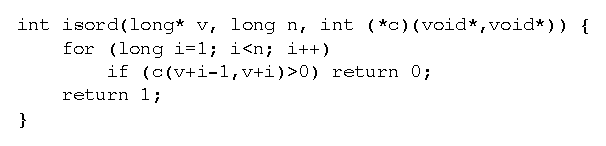
\includegraphics[width=0.9\columnwidth]{figures/isord-example/isord.eps}
\caption{\protect\label{fig:isordfrom} OSR instrumentation of base function in LLVM IR (in grey). The OSR is fired at the beginning of the loop body after 1000 iterations.
}
\end{center}
\end{figure}
\fi

\ifdefined\noauthorea
\begin{figure}[t]
\begin{center}
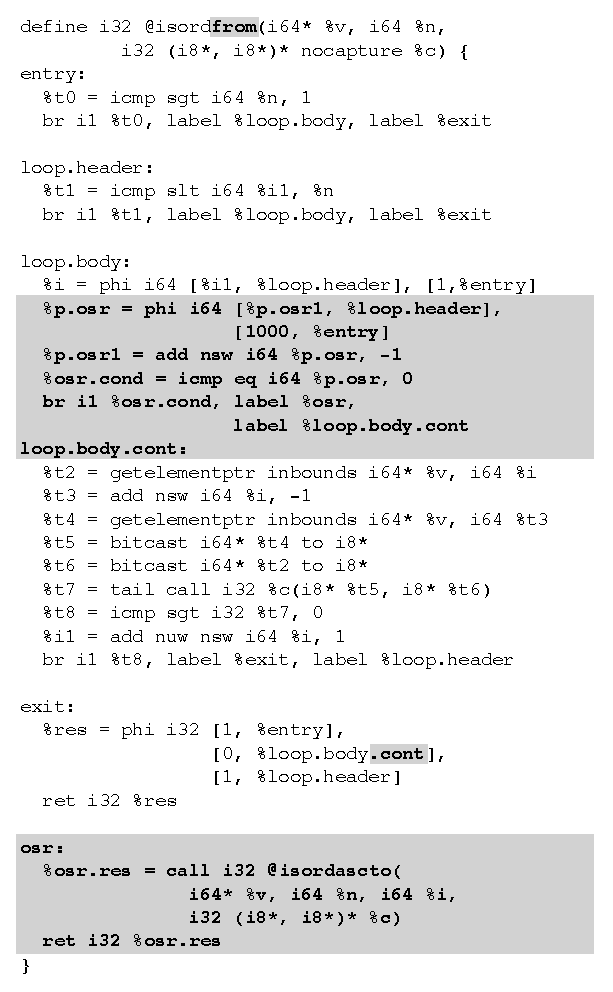
\includegraphics[width=0.9\columnwidth]{figures/isordfrom/isordfrom.eps}
\caption{\protect\label{fig:isordfrom} IR version of base function {\tt isord} (\myfigure\ref{fi:isord-example}) instrumented for resolved OSR. The OSR is fired at the beginning of the loop body after 1000 iterations. Additions resulting from the instrumentation are in grey.
}
\end{center}
\end{figure}
\fi

\ifdefined\noauthorea
\begin{figure}[t]
\begin{center}
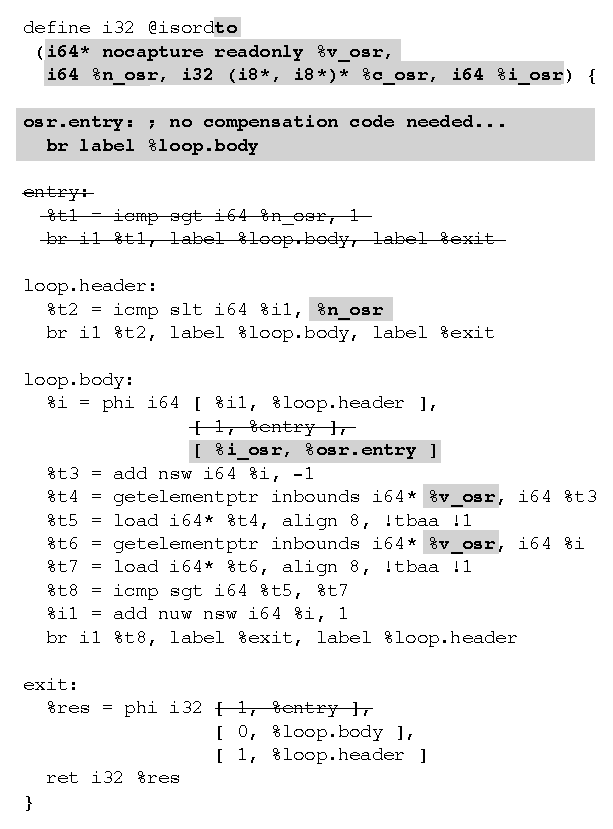
\includegraphics[width=0.9\columnwidth]{figures/isordascto/isordascto.eps}
\caption{\protect\label{fig:isordascto} OSR instrumentation (in grey) of faster variant {\tt isordasc} (\myfigure\ref{fi:osr-dynamics}) in LLVM IR. The original function entry block is unreachable after instrumentation and eliminated (struck-through code fragments).
}
\end{center}
\end{figure}
\fi

\subsection{Resolved OSR Points}

\subsection{Open OSR Points}
  
%\begin{verbatim}
%int fac(int n) {
%    int i = 2, f = 1;
%    while (i<=n) f *= i++;
%    return f;
%}
%\end{verbatim}
%
%\begin{verbatim}
%int fac(int n) {
%    int i = 2, f = 1;
%    while (i<=n)  {
%        if (osr_cond) return fac_osr(n,i,f); 
%        f *= i++; 
%    } return f;
%}
%\end{verbatim}
%
%\begin{verbatim}
%int fac_osr(int n) {
%    goto L;
%    int i = 2, f = 1;
%    while (i<=n) L: f *= i++;
%    return f;
%}
%\end{verbatim}


  
  
  
  
  